\documentclass[norsk,a4paper,12pt]{article}
\usepackage[T1]{fontenc} %for å bruke æøå
\usepackage[utf8]{inputenc}
\usepackage{graphicx} %for å inkludere grafikk
\usepackage{verbatim} %for å inkludere filer med tegn LaTeX ikke liker
\usepackage{mathpazo}
\usepackage{amsmath}
\usepackage{flafter} % skal tydeligvis gjøre at figurer havner i riktig kronologisk rekkefølge i forhodl til teksten
\usepackage[titletoc]{appendix}
\renewcommand{\arraystretch}{1,5}
\bibliographystyle{plain}
\usepackage{natbib}
\linespread{1.1}

\newcommand{\figurewidth}{10cm}

\newcommand{\textdirectcurrent}{%
  \settowidth{\dimen0}{$=$}%
  \vbox to .85ex {\offinterlineskip
    \hbox to \dimen0{\leaders\hrule\hfill}
    \vskip.35ex
    \hbox to \dimen0{%
      \leaders\hrule\hskip.2\dimen0\hfill
      \leaders\hrule\hskip.2\dimen0\hfill
      \leaders\hrule\hskip.2\dimen0
    }
    \vfill
  }%
}
\newcommand{\mathdirectcurrent}{\mathrel{\textdirectcurrent}}

\title{Labrapport Vekselstrømskretser - FYS2150}
\author{Ditt navn}
\date{\today}
\begin{document}

\maketitle

\begin{abstract}
Hensikten med labben er å bli kjent med bruk av oscilloskop og dets tilhørende programmvare. I tillegg sammenligner vi det met et multimeter. Vi undersøker målinger av RMS-verdier og finner at multimeter ved høye frekvenser grunnet bruker av likeretter (bridge rectifier) ikke klarer å lade/utlade hurtig nok slik at RMS-verdien blir for liten. Videre undersøker vi en krets bygd opp av en resistand og en induktans i serie. Induktansen finner vi først ved å anta null resistans og måler diverse størrelser på coil og leder. Deretter ved bruk av lineærregresjon til spenningene over komponentene sammen og spenningen over resistoren. Finner henholdsvis en verdi for L på omtrent 0.86 og 0.77 mH som forskjellen ligger innenfor den totale usikkerheten utregnet til 0.17. Avsluttende undersøker vi hvordan frekvensen påvirker effekten i et øyeblikk og over en periode. Finner at når frekvensen øker, så vil fasen øke opp mot 90 grader som igjen minker effekten som er lett synlig i det teoretiske utrykket ved bruk av cos. 

\end{abstract}

\section{Introduksjon}
Målet i denne oppgaven er å bli kjent med et oscilloskop og bruke det til å måle på vekselstrømkretser. Vi er ute etter å måle RMS verdien for to ulike signaler og sammenligne med den teoretiske verdien.  Deretter undersøker vi en “hjemmelaget” krets. Vi bruker en Pico-modul for å generere signalet vårt. Vi målet spenning gjennom en kombinasjon av å bruke et multimeter og oscilloskop som kobles opp til PC-en hvor vi justerer frekvensen og signaltype. Kretsen består av en spenningskilde, induktor og en konstant motstand. Vi ønsker å undersøke hva som skjer med induktoren når vi varierer frekvensen og finne induktansen ved to ulike metoder. Til slutt ser vi nærmere på faseforskyvning grunnet induktoren. Hvordan varierer fasen med frekvens og hva skjer med effekten når faseforskyvningen øker. Vi ønsker å se på hvor perfekt induktoren oppfører seg.


\section{Teori}


For å forstå fremgangen og resultater i oppgaven er det en del viktige begreper:

\begin{itemize} 
\item Likestrøm vs vekselstrøm: Likestrøm (DC) er en konstant, enveis strøm. Vekselstrøm (AC) endrer periodisk retning og størrelse. Vi tar i bruk AC, siden det vil gi endring i strømmen som fører til indusert spenning.
\item Effektivverdi (RMS): Effektivverdien til et vekselstrømssignal er en måleenhet for verdien som tilsvarer likestrømsverdien som ville produsert samme varmeeffekt. Veriden kan vi finne teoretisk. RMS er en statistisk middelverdi av et sett med tall eller måleserie av en variabel og defineres som kvadratroten av gjennomsnittet av verdiene kvadrert.

%RMS eq
\begin{equation}
V_{RMS}=\sqrt{\frac1{T_{2}-T_{1}}\int_{T_{1}}^{T_{2}}[V(t)]^{2}dt}\\
\label{eq: RMS vekselstrøm}
\end{equation}
hvor T1 og T2 er start- og sluttidspunktet for målingen.

For en sinusbølge og firkantbølge er verdien lik:
%RMS sinus og firkant
\begin{equation}
RMS_{sinus}=\frac{A}{\sqrt{2}} \approx 0.707*A \\
\label{eq: RMSsin}
\end{equation}


\begin{equation}
RMS_{firkant}= {A} \\
\label{eq: RMSsq}
\end{equation}
hvor A er amplituden, som i denne sammenhengen er spenningen V0.

\item Faseforskyvning : Faseforskyvning refererer til forskyvningen i timingen eller fasen til et vekselstrømssignal i forhold til et annet signal. For oss vil det våre fasen mellom spenningen målt over to ulike områder i kretsen. 

\item Lenz lov: Lenz lov sier at retningen til en indusert strøm i en leder er slik at den motvirker endringen i det magnetiske feltet som produserte den. F.eks om vi øker strømmen langs spole vil det bli indusert en spenning som vil skape en motsetning i strømmen.

\item Induktor: En induktor er en elektronisk komponent som lagrer energi i sitt magnetiske felt, i vårt tilfelle er den en del av en enkel RL-krets (resistor og induktor krets). Vil motvirke endringer i endringer av strøm i kretsen.

\item Induktans: Induktans er en egenskap ved en induktor og representerer dens evne til å lagre energi i form av et magnetfelt. For en spole med d N vindinger er induktansen L definert
som:  
\begin{equation}
L=\frac{N\Phi_{B}}{I}
\label{eq: Induktans}
\end{equation}
Hvor I er strømmen og $\Phi$ er den gjennomsnittlige magnetiske fluksen gjennom hver vinding. 

Ved å bruke utrykkene: magnetisk flukstetthet ($B=\frac{\mu_0NI}l$), fluksen ($\Phi_B=\frac{\mu_0}l\pi r^2$, hvor $\mu_0$ er den magnetiske permeabiliteten i vakuum, også kjent som vakuums permeabilitet. Verdien vi tar i bruk er $1.256637e-6$ ) og utrykket for vindinger N ved lederlendge $\lambda$ ($N=\frac\lambda{2\pi r}$). Vi utnyttet at tråden har en motstand per meter k =
0.3547 ± 0.0004$\Omega$ per meter. Ved litt omrokeringer ender vi med et utrykk: 

%Induktans final
\begin{equation}
L=\frac{\mu_{0}\lambda^{2}}{4\pi l}\\
\label{eq: induktansen}
\end{equation}

Dette er uavhengig av radiusen r og vil være en approksimasjon og antar en perfekt spole med homogen flukstetthet.  I virkeligheten er den svakere ved endene av solenoiden. Ved mindre spole, vil det gi større relativ feil. \\

Den selvinduserte emf, $\varepsilon$ , blir:
%Selvinduserte emf 
\begin{equation}
V_L = \varepsilon=-L\frac{dI}{dt}\\
\label{eq: emf}
\end{equation}
Ved å bruke utrykket for strøm $I(t)=I\mathrm{cos}(\omega t)\mathrm{mht}$ og differensierer dette får vi: $V_L=-\omega Llsin(\omega t)=\omega Llcos(\omega t+90^\circ)$. Dette er en 90 graders faseforskyvning i forhold til strømmen. Dette er for en ren induktor(uten ohmisk motstand), men fasen vil være 0 for en ren motstand. I virkeligheten har enhver spole en viss motstand fordi kobberledninger har en resistivitet, så induktoren kan ses som en motstand og en ren induktor i seriekobling. Den vil ikke nå 90 grader men vil nærme seg, viktig å nevne at den ikke heller kan overstride 90. Vi får da et utrykk for spenning lik: 
%Spenning med fase:
\begin{equation}
V_L=\omega LI\cos(\omega t+\phi)\\
\label{eq: }
\end{equation}
hvor faseforskyvningen er lik $\phi=\tan^{-1}(\frac{\omega L}R)$


\item Impedans: Måleenhet på hvor mye en komponent i en elektrisk krets motsetter seg strømmen når en spenning påføres. Oppgis vanligvis i enhethen ohm. I denne RL-kretsem får vi impedans (Z) lik: 
%Z squared: 
\begin{equation}
Z^2=R^2+\omega^2L^2=\left(\frac{V_A}I\right)^2,\mathrm{og~}I=\frac{V_R}R.
\label{eq: Z_Impedans}
\end{equation}
hvor Z er impedansen og vinkelhastigheten, betegnet med $\omega$, er definert ved formelen $\omega = 2\pi f$, hvor $f$ er frekvensen i hertz (Hz).

\item Reaktans: Delen av impedansen som er grunnet i induktansen og kapasitansen. \cite{snl_reaktans} Måles i ohm. Er det som forårsaker faseforskyvningen i kretsen. I en induktor kan vi utrykke det som:  $X_L=\omega L$. Vi ser at når frekvensen øker, vil reaktansen øke og faseskiftet går mot den teoretiske grensen på 90 grader. Ved likestrøm vil den naturligvis være null. 

\item Usikkerheter: For å finne usikkerheter i utregningeer av blant annet induktansen L bruker vi en generell formel lik ved ganging og deling: 

\begin{equation}
    \left(\frac{\Delta Z}Z\right)^2=\left(\frac{\Delta A}A\right)^2+\left(\frac{\Delta B}B\right)^2
    \label{eq: errorGange}
\end{equation}
hvor verdien Z er en funksjon av verdiene A og B. Tas i bruk for feil til utregning av induktans og lengde. For sammensatte usikkerheten bruker vi formel for usikkerhet når vi adderer og subtraherer.

\begin{equation}
    \left(\Delta Z\right)^2=\left(\Delta A\right)^2+\left(\Delta B\right)^2
    \label{eq: errorPluss}
\end{equation}

Formler hentet fra Squires s.29 \cite{squires1985}.



\item Lineær tilpasning: Lineær tilpasning er en metode brukt for å finne den best tilpassede lineære sammenhengen mellom to variabler. Det innebærer å finne stigningen og skjæringspunktet til linjen som best beskriver dataene. I del 2 av oppgaven får vi bruk for dette når vi tar utgangspunkt i likning \ref{eq: Z_Impedans} med litt omrokeringer får vi utrykket: 
\begin{equation}
\left(\frac{V_A}{V_R}\right)^2=\frac{L^2}{R^2}\omega^2+1
\label{eq: V_a over V_r}
\end{equation}


\item Effekt og effektavsetning: En fysisk størrelse definert som omsatt energi per tidsenhet og målet i watt I SI-enhetet. I den elektriske kretsen er effekt lik produktet av spenning og strømmen. For en ren motstand med null faseforskyvning får vi effekt lik: %Ekkefkt / Power: 0 grader
\begin{equation}
P=I(t)V(t)=IV\cos^2(\omega t)\\
\label{eq: }
\end{equation}

Gjennomsnittsverdien for $cos^2(\omega t)$ er lik 0.5, da får vi gjennomsnittseffekt lik: 
%Psnitt
\begin{equation}
P_{snitt}=\frac12IV=\frac1{\sqrt2}\frac1{\sqrt2}IV=I_{rms}V_{rms}\\
\label{eq: }
\end{equation}

Hvis vi legger til faseforskyvning blir utrykket for P lik: 
%P ved faseforskyvning
\begin{equation}
\begin{split}
P & =I(t)V(t)=Icos(\omega t)Vcos(\omega t+\phi)) \\
 & =V(\cos(\omega t)\cos(\phi) -\sin(\omega t)\sin(\phi) (l\cos(\omega t)) 
\end{split}
\label{P_fase}
\end{equation}

Gjennomsnittsverdien av   $cos(\omega t)*sin(\omega t)$ er lik null og
gjennomsnittsverdien av  $cos^2(\omega t)$ er igjen 0.5. Da ender vi til slutt opp med et endelig utrykk for snitt verdien av effekten: 
%Psnitt final phase
\begin{equation}
P_{snitt}=I_{rms}V_{rms}\cos(\phi)
\label{eq: P_snitt}
\end{equation}
Fra cos funksjonen ser vi raskt at ved 90 grader vil utrykket bli 0, og ved null grader vil bare være lik $V*I$.


\end{itemize}

\section{Eksperimentelt}
Utstyrsliste(hentet fra oppgavetekst):
\begin{itemize} 
\item Ett Håndholdt multimeter (FLUKE 75)  \item Oscilloskop med innebygd signalgenerator (PicoScope 2000 Series) \item PC med PicoScope-programvaren installert \item Løse ledninger (enkeltledere) \item 1 Koaks-kabel med BNC i hver ende \item 3 Koaks-kabler med banan \item 2 ledninger med klype \item 1 BNC-T overgang \item 100 Ω motstand \item Plastsylinder med kobbertråd-spole (induktor) \item Skyvelære \item Kretskort for RL- og RC-kretser 
\end{itemize}

(Skisser og nøyaktigheter til måleutstyr)
\subsection{Vekselspenning med frekvensgenerator, oscilloskop og multimeter }
Vi ønsket å undersøke hvordan vi måler spenningen med et multimeter og et oscilloskop (PicoScope
2000 series). Ved bruk av disse to kan vi undersøke signalets RMS verdi for ulike former på signalet. Oppsett vist i figur \ref{fig:opg1_oppsett}, vi bruker en koaks-kabel til å koble direkte fra utgangen
AWG til inngang A på skopet og bruker en splitter "BNC T" for å legge til et multimeter slik at vi kan måle spenningen samtidig. Signalgeneratoren settes på frekvens lik 1 kHz og spenning på 1 V. Setter på AC spenning. Vi tok i bruk innstillinger gitt fra APPENDIKS A som gir et godt bilde vist på monitoren i PicoScope programmet. Mangler bildet av induktor, men vil være lik form som vist i fig \ref{fig: spole} \\


\begin{figure}[htbp]
    \centering
    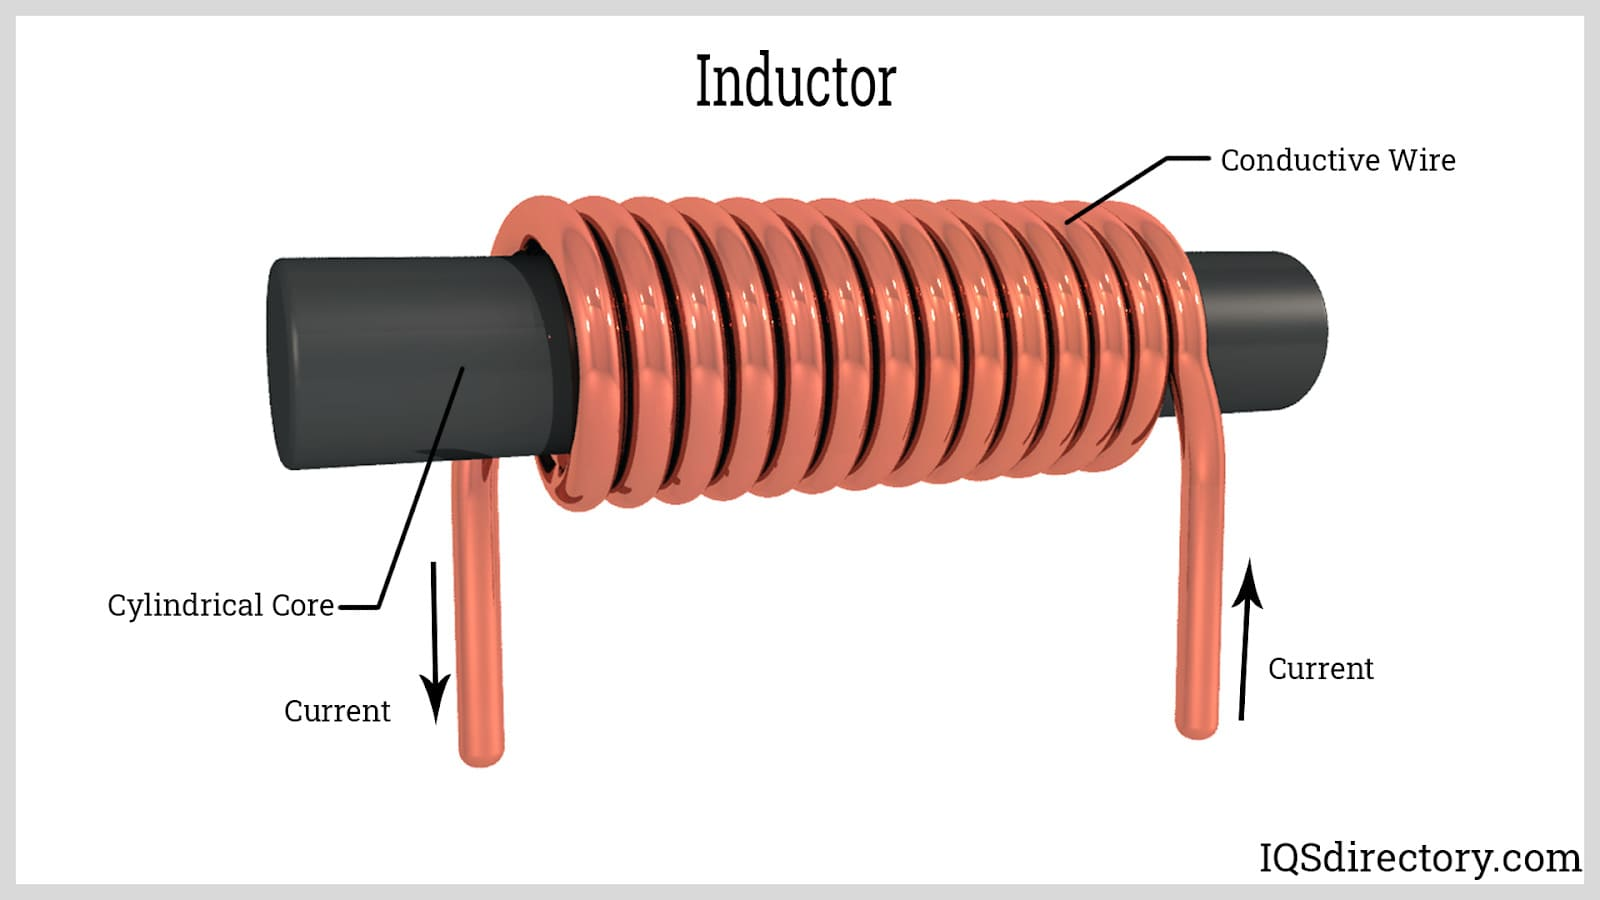
\includegraphics[width=0.7\textwidth]{Figs/inductor.jpg}
    \caption{En kobbertråd som er spunnet rundt en sylinder av plast som vil induktoren i kretsen. Source: \cite{InductorCoils2023}}
    \label{fig: spole}
\end{figure}


Starter med signal type like sinusbølge. Vi velger verktøy i programmet og legger til måling av AC RMS for spenningen på inngang A. Dette gir sanntids evaluering av RMS verdien og vil være veldig presis så lenge vi har tilstrekkelig perioder og at signalet ikke klipper ut av bildet (som vist i figur \ref{fig:sinwave} i resultater). I tillegg til sinusbølgen, ønsker vi også å undersøke en firkantbølge. For begge bølgene velger vi å variere frekvensen til fire ulike verdier: 50 Hz, 500 Hz, 1000 Hz og 5000 Hz. Vi noterer ned verdiene som multimeteret og oscilloskopet viser. For sinusbølgen gjør enda en undersøkelse hvor vi legger til en DC-komponent til signalet, som resulterer av en forskyvning av signalet i den vertikale aksen. Deretter prøver vi å finne to ulike måter å måle denne forskyvningen ved hjelp av multimeteret og oscilloskopet. 



\subsection{Induktor og RL-krets}
I den andre delen ønsker vi å anslysere en enkel RL-krets og dens atferd ved varierende frekvens. Vi er også ute etter å finne induktansen på to ulike måter. Først måler vi resistansen ved bare å plugge inn induktoren direte til multimeteret, multimeteret har litt innebygd spenning slik et ny spenningskilde ikke er nødvendig ved bare måling av resistans. Vi bruker et enkelt kretskort og tar utgangspunkt i oppsett i figur \ref{fig:krets} hvor vi har et signal, igjen generert av Pico modulen, og en resistor pluss en induktor. På grunn av råd/anbefaling grunnet måten kretsene var bygd opp på, valgte vi å modifisere oppsettet litt slik av vi heller måle spenningen over begge komponentene istedenfor bare spolen. Vi fortsetter også å måle separat spenningen over resistoren som vist i figur \ref{fig:krets_mod}. Spolen var bygd opp av en kobbertråd som var spunnet rundt en sylinder og motstanden i denne kretsen var på 100 ohm.  \\

Etter kretsen er satt opp og vi har input koblet opp til Pico modulen og inn igjen til PC-en slik at vi ser nå to signaler. Den ene har vi kalt for V\_a som er spenningen over hele kretsen, mens V\_b er spenningen over resistoren som vi i sanntid måler ved igjen bruk av RMS målingen i Pico programmet. Signalene vil ikke være helt i fase, derfor ved hjelp av verktøy i programmet måler vi fasen ved å følge instruksjonene: nederst til høyre i plottet finnes en blå runding. Den kan trekkes 2 ganger til to påfølgende toppunkter på den ene kurven (angir perioden). Deretter trekkes med den hvite firkant nederst til venstre en linje til den andre kurven og vinkelen kan avleses. Alle 3 målingene, to spenninger(mV) og fase, måles i det vi endrer frekvensen. Vi gjør dette for 7 ulike frekvenser (400, $10^3$, $50 \times 10^3$, $100 \times 10^3$, $200 \times 10^3$, $300 \times 10^3$, $400 \times 10^3$) Hz. Dette for den andre metoden å finne induktansen, L, på. \\

Videre ønsker vi å utforske effektavsetningen. Hvor vi utnytter at spenningene multiplisert er proporsjonal med avsetningen. I programmet velger vi verktøy og viser likestrømsgjennomsnitt for kanalene multiplisert A*B , hvor vi noterer ned 6 verdier for ulike frekvenser $(5 \times 10^3, 20 \times 10^3, 30 \times 10^3, 40 \times 10^3, 50 \times 10^3, 60 \times 10^3, 70 \times 10^3, 80 \times 10^3)$. Vi bruker dette senere når vi skal plotte effekt gjennomsnittet mot den teoretiske verdien vist i ligning \ref{eq: P_snitt}.



\begin{figure}[htbp]
    \centering
    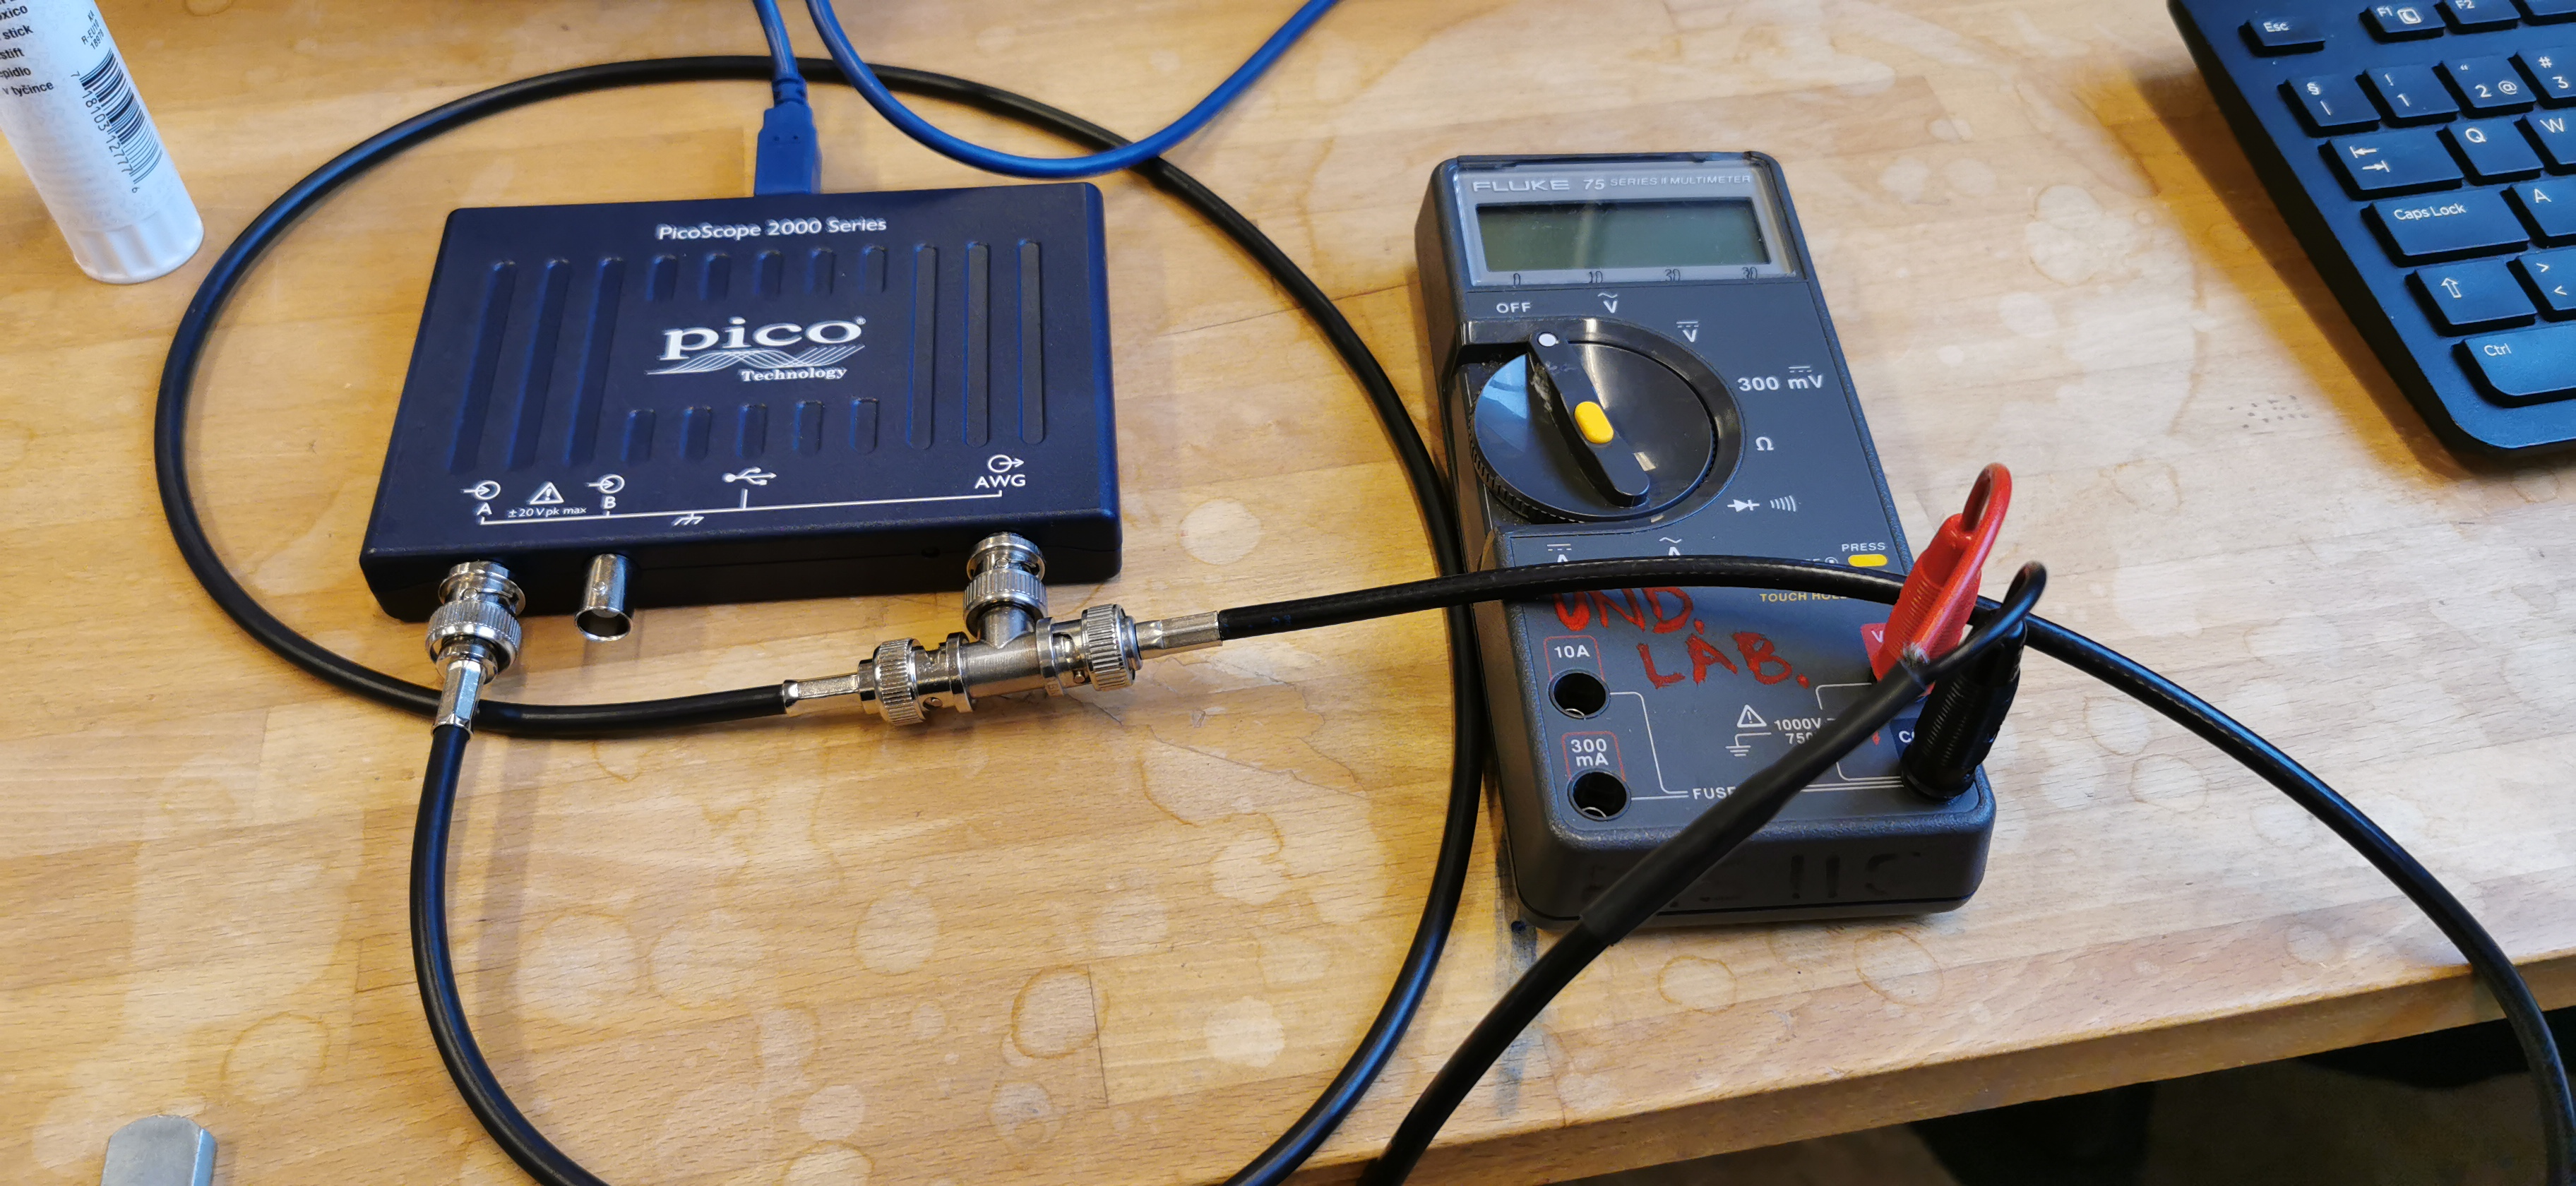
\includegraphics[width=1\textwidth]{Figs/Opg1.jpg}
    \caption{Oppsett for måling av volt gjennom multimeter og oscilloskop}
    \label{fig:opg1_oppsett}
\end{figure}


\begin{figure}[htbp]
    \centering
    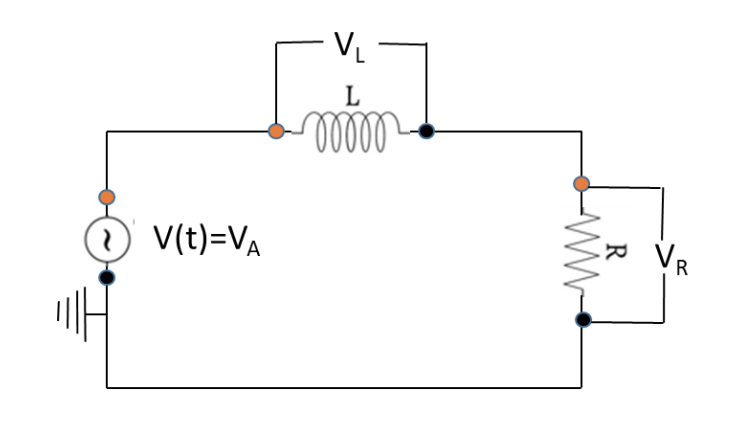
\includegraphics[width=\figurewidth]{Figs/skjema.png}
    \caption{Startoppsett for kretsen. Vi bruker en variasjon av denne }
    \label{fig:krets}
\end{figure}

\begin{figure}[htbp]
    \centering
    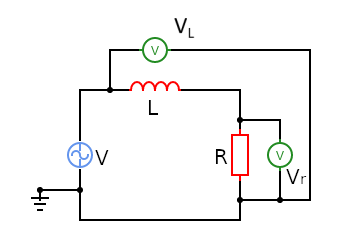
\includegraphics[width=\figurewidth]{Figs/circuit.png}
    \caption{ Modifiserte oppsettet, V\_L måler over begge komponenter. V\_r måler spenning over en motstand på 100 ohms. Spenningskilden vil være på typen AC og vil ha en frekvens bestemt i Pico programmet. }
    \label{fig:krets_mod}
\end{figure}

I første oppgave tar vi i bruk multimeter og oscillator. Multimeteret, FLUKE75, tas i bruk på innstillingen vekselstrøm mV$\sim$(AC strøm). Avlesning av datablad viser at vi har en rekkevidde på 320 mV, en oppløsning på 0.1 mV og en nøyaktighet på $\pm(2\% + 2)$. Vi velger å se bort fra Picoscopets nøyaktighet, med tanke på det er så presist i forhold til multimeteret og usikkerhet rundt nøyaktig hvilken verdi å velge fra databladet.
For skyvevære vi brukte til å måle lengde til delen av induktoren spunnet rundt sylinderen. Vi regner med nøyaktighet på 0.05 mm. For oppgave 2, når vi måler resistansen har vi en nøyaktig på $\pm(0.5\% + 2)$. 


%\clearpage % fix figure chaos


\section{Resultater}
\subsection{Del 1}
Ved måling av RMS verdien gjennom multimeter og oscilloskop for fire ulike frekvenser fikk vi verdiene vist i tabell \ref{tab:Fig1} for sinusbølge. Tilsvarende for firkantsignalet fikk vi verdier presentert i tabell \ref{tab:Fig2}. Signalet som vist gjennom programvaren til PicoScopet er vist for sinus og firkantsignal i figur \ref{fig:sinwave} og figur \ref{fig:sq_wave}. For en måling på 0.707V med multimeter gir det en feil med tre gjeldende siffer lik 0.016V (likning fra eksperimentelt/datablad for multimeter). 

\begin{table}[htbp]
    \centering
    \caption{Sinusbølge spenning målt med multimeter og oscilloskop. Signal generert av PicoScope på 1V. Teoretisk verdi: $RMS=\sqrt{\frac{A^{2}}{2}}\approx.707A$}
    \begin{tabular}{lll}
     \hline
     \textbf{Frekvens $f$ [Hz]} & \textbf{Multimeter $V_m$ [V]} & \textbf{PicoScope $V_0$ [V]}  \\
     \hline
     $50$Hz & $0.703$V & $0.707$V \\
     \hline
     $500$Hz & $0.700$V & $0.707$V \\
     \hline
     $1000$Hz & $0.690$V & $0.707$V \\
     \hline
     $5000$Hz & $0.496$V & $0.707$V \\
     \hline
     & 
\end{tabular}
    \label{tab:Fig1}
\end{table}

\begin{table}[htbp]
    \centering
    \caption{Firkantbølge spenning målt med multimeter og oscilloskop. Signal generert av PicoScope på 1V. Teoretisk verdi: $V\_RMS = A = V_0$ }
    \begin{tabular}{ccc}
     \hline
     \textbf{Frekvens $f$ [Hz]} & \textbf{Multimeter $V_m$ [V]} & \textbf{PicoScope $V_0$ [V]}  \\
     \hline
     $50$Hz & $1.10$V & $0.997$V \\
     \hline
     $500$Hz & $1.06$V & $0.997$V \\
     \hline
     $1000$Hz & $1.01$V & $0.995$V \\
     \hline
     $5000$Hz & $0.644$V & $0.994$V \\
     \hline
     & 
    \end{tabular}
    
    \label{tab:Fig2}
\end{table}

\begin{figure}[htbp]
    \centering
    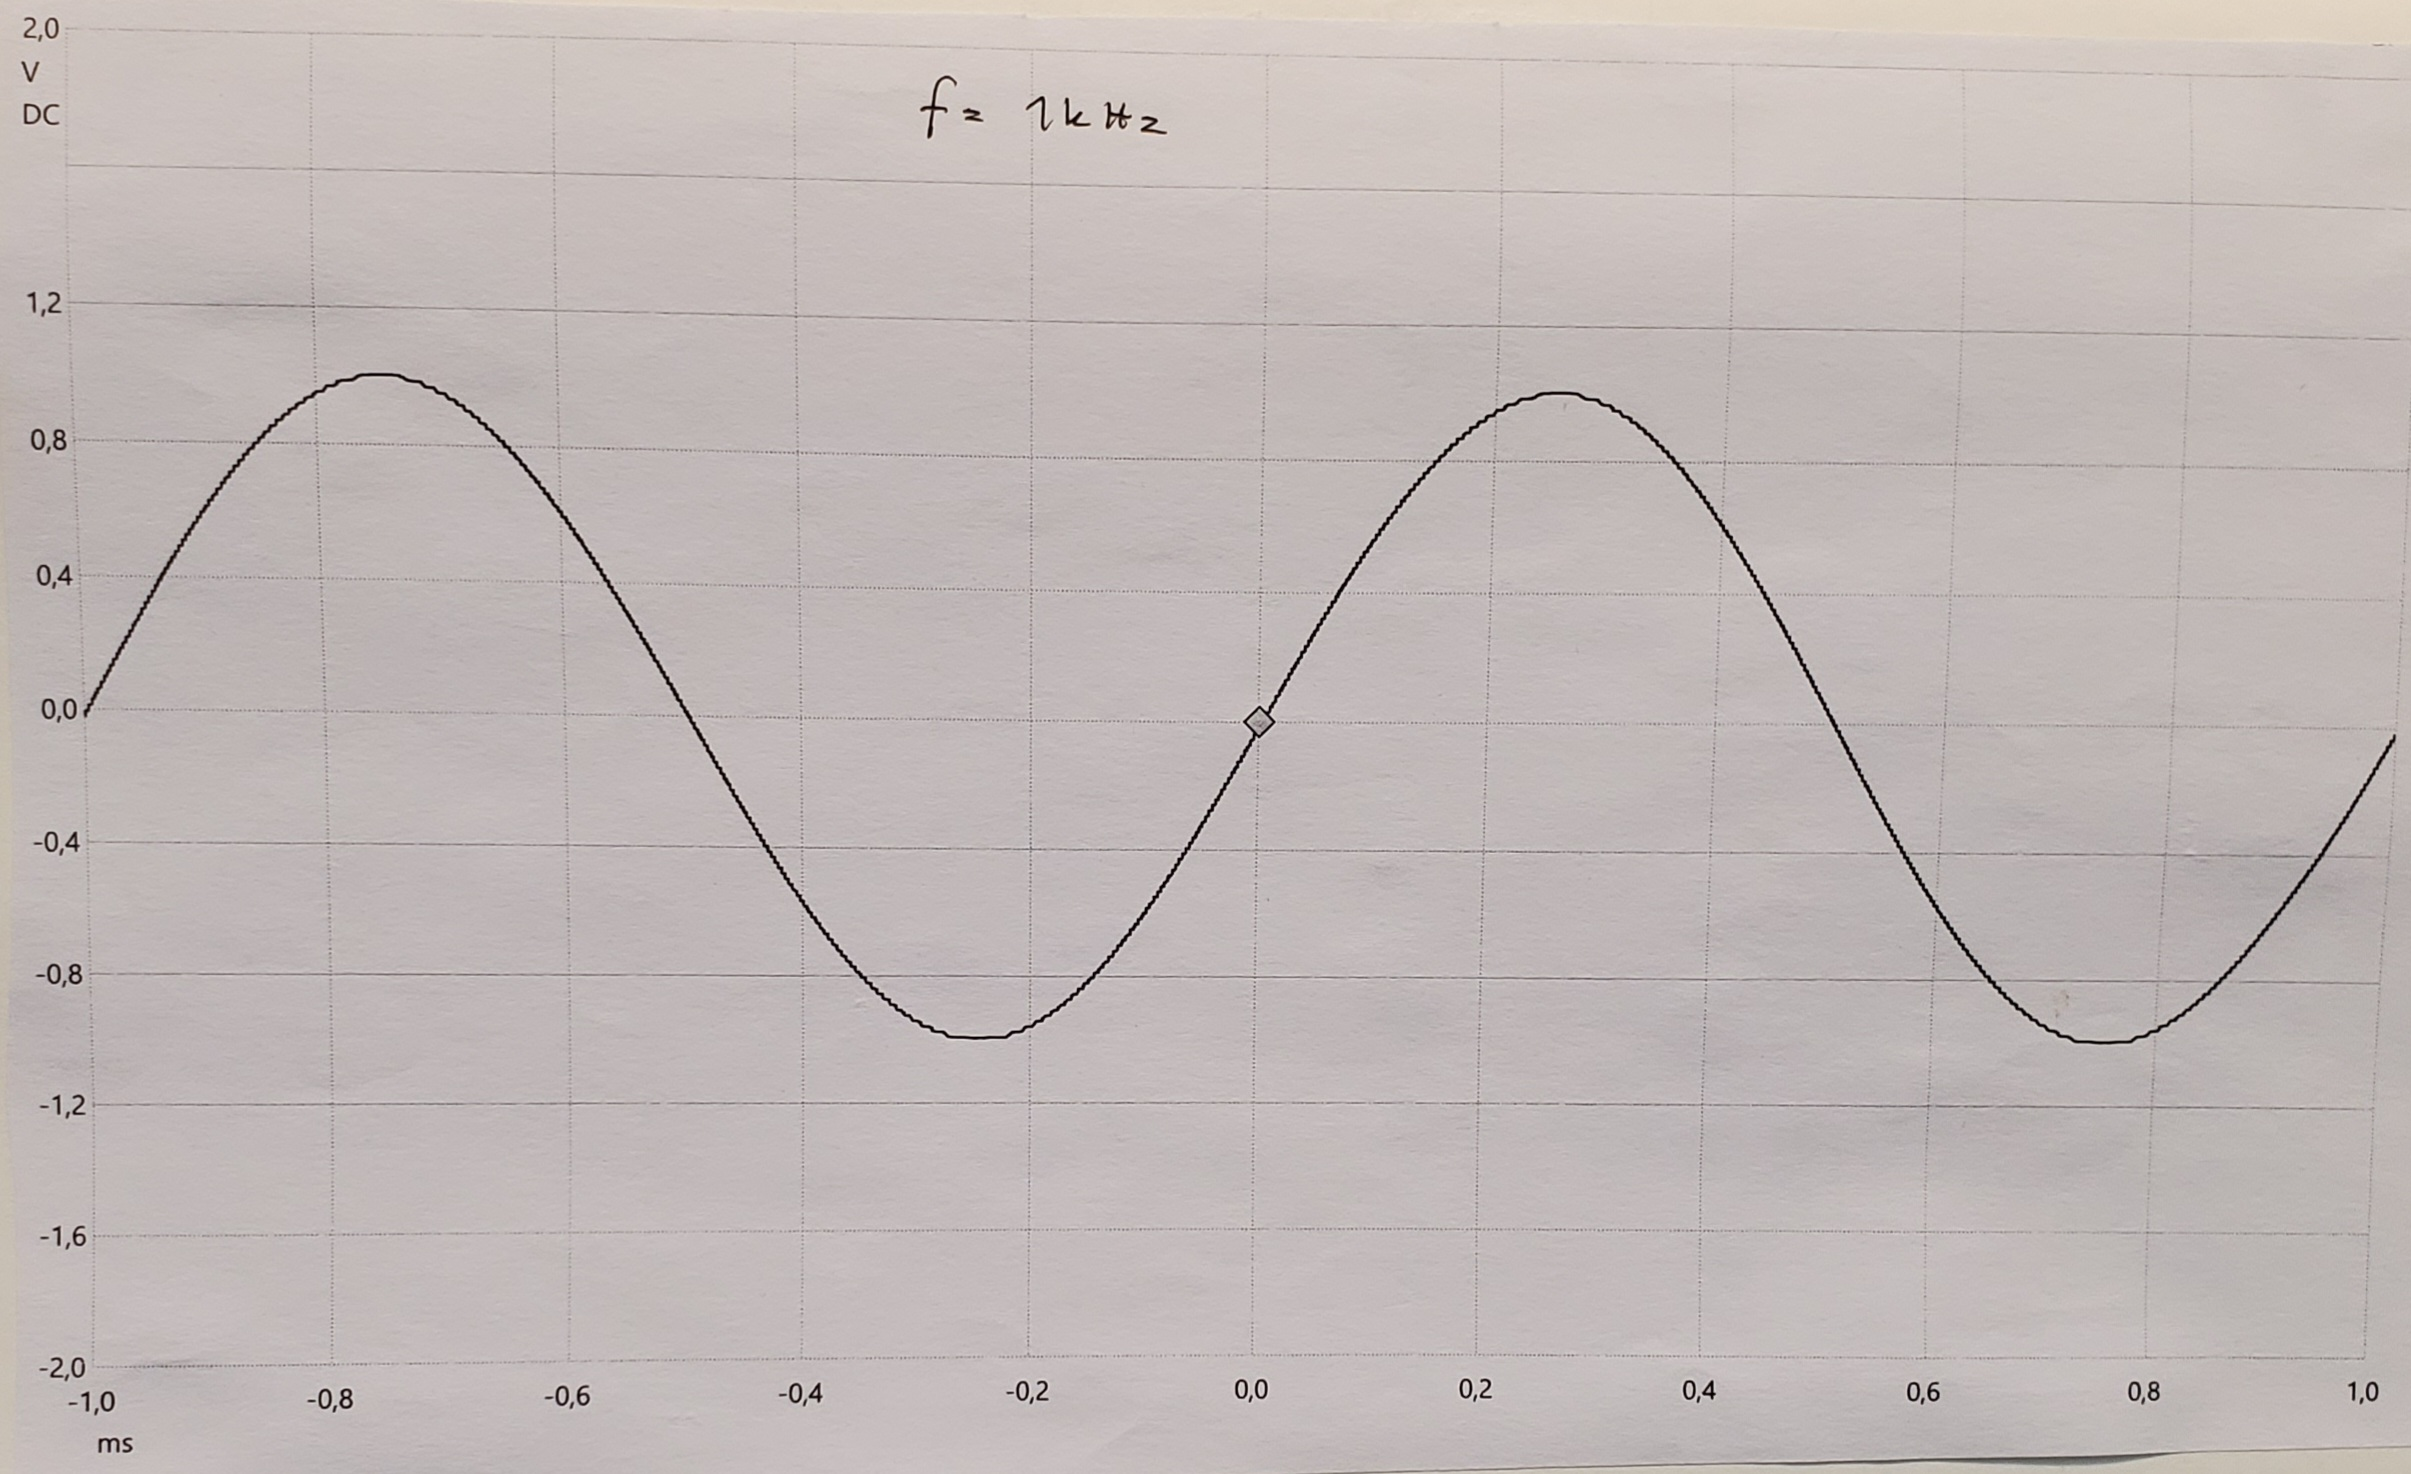
\includegraphics[width=1\textwidth]{Figs/sinussignal.jpg}
    \caption{Sinussignal som vist i PiscoScope 6 ved 1 volt og frekvens lik 50 Hz. Spenning(V) mot tid(ms). Oppgave 1}
    \label{fig:sinwave}
\end{figure}

\begin{figure}[htbp]
    \centering
    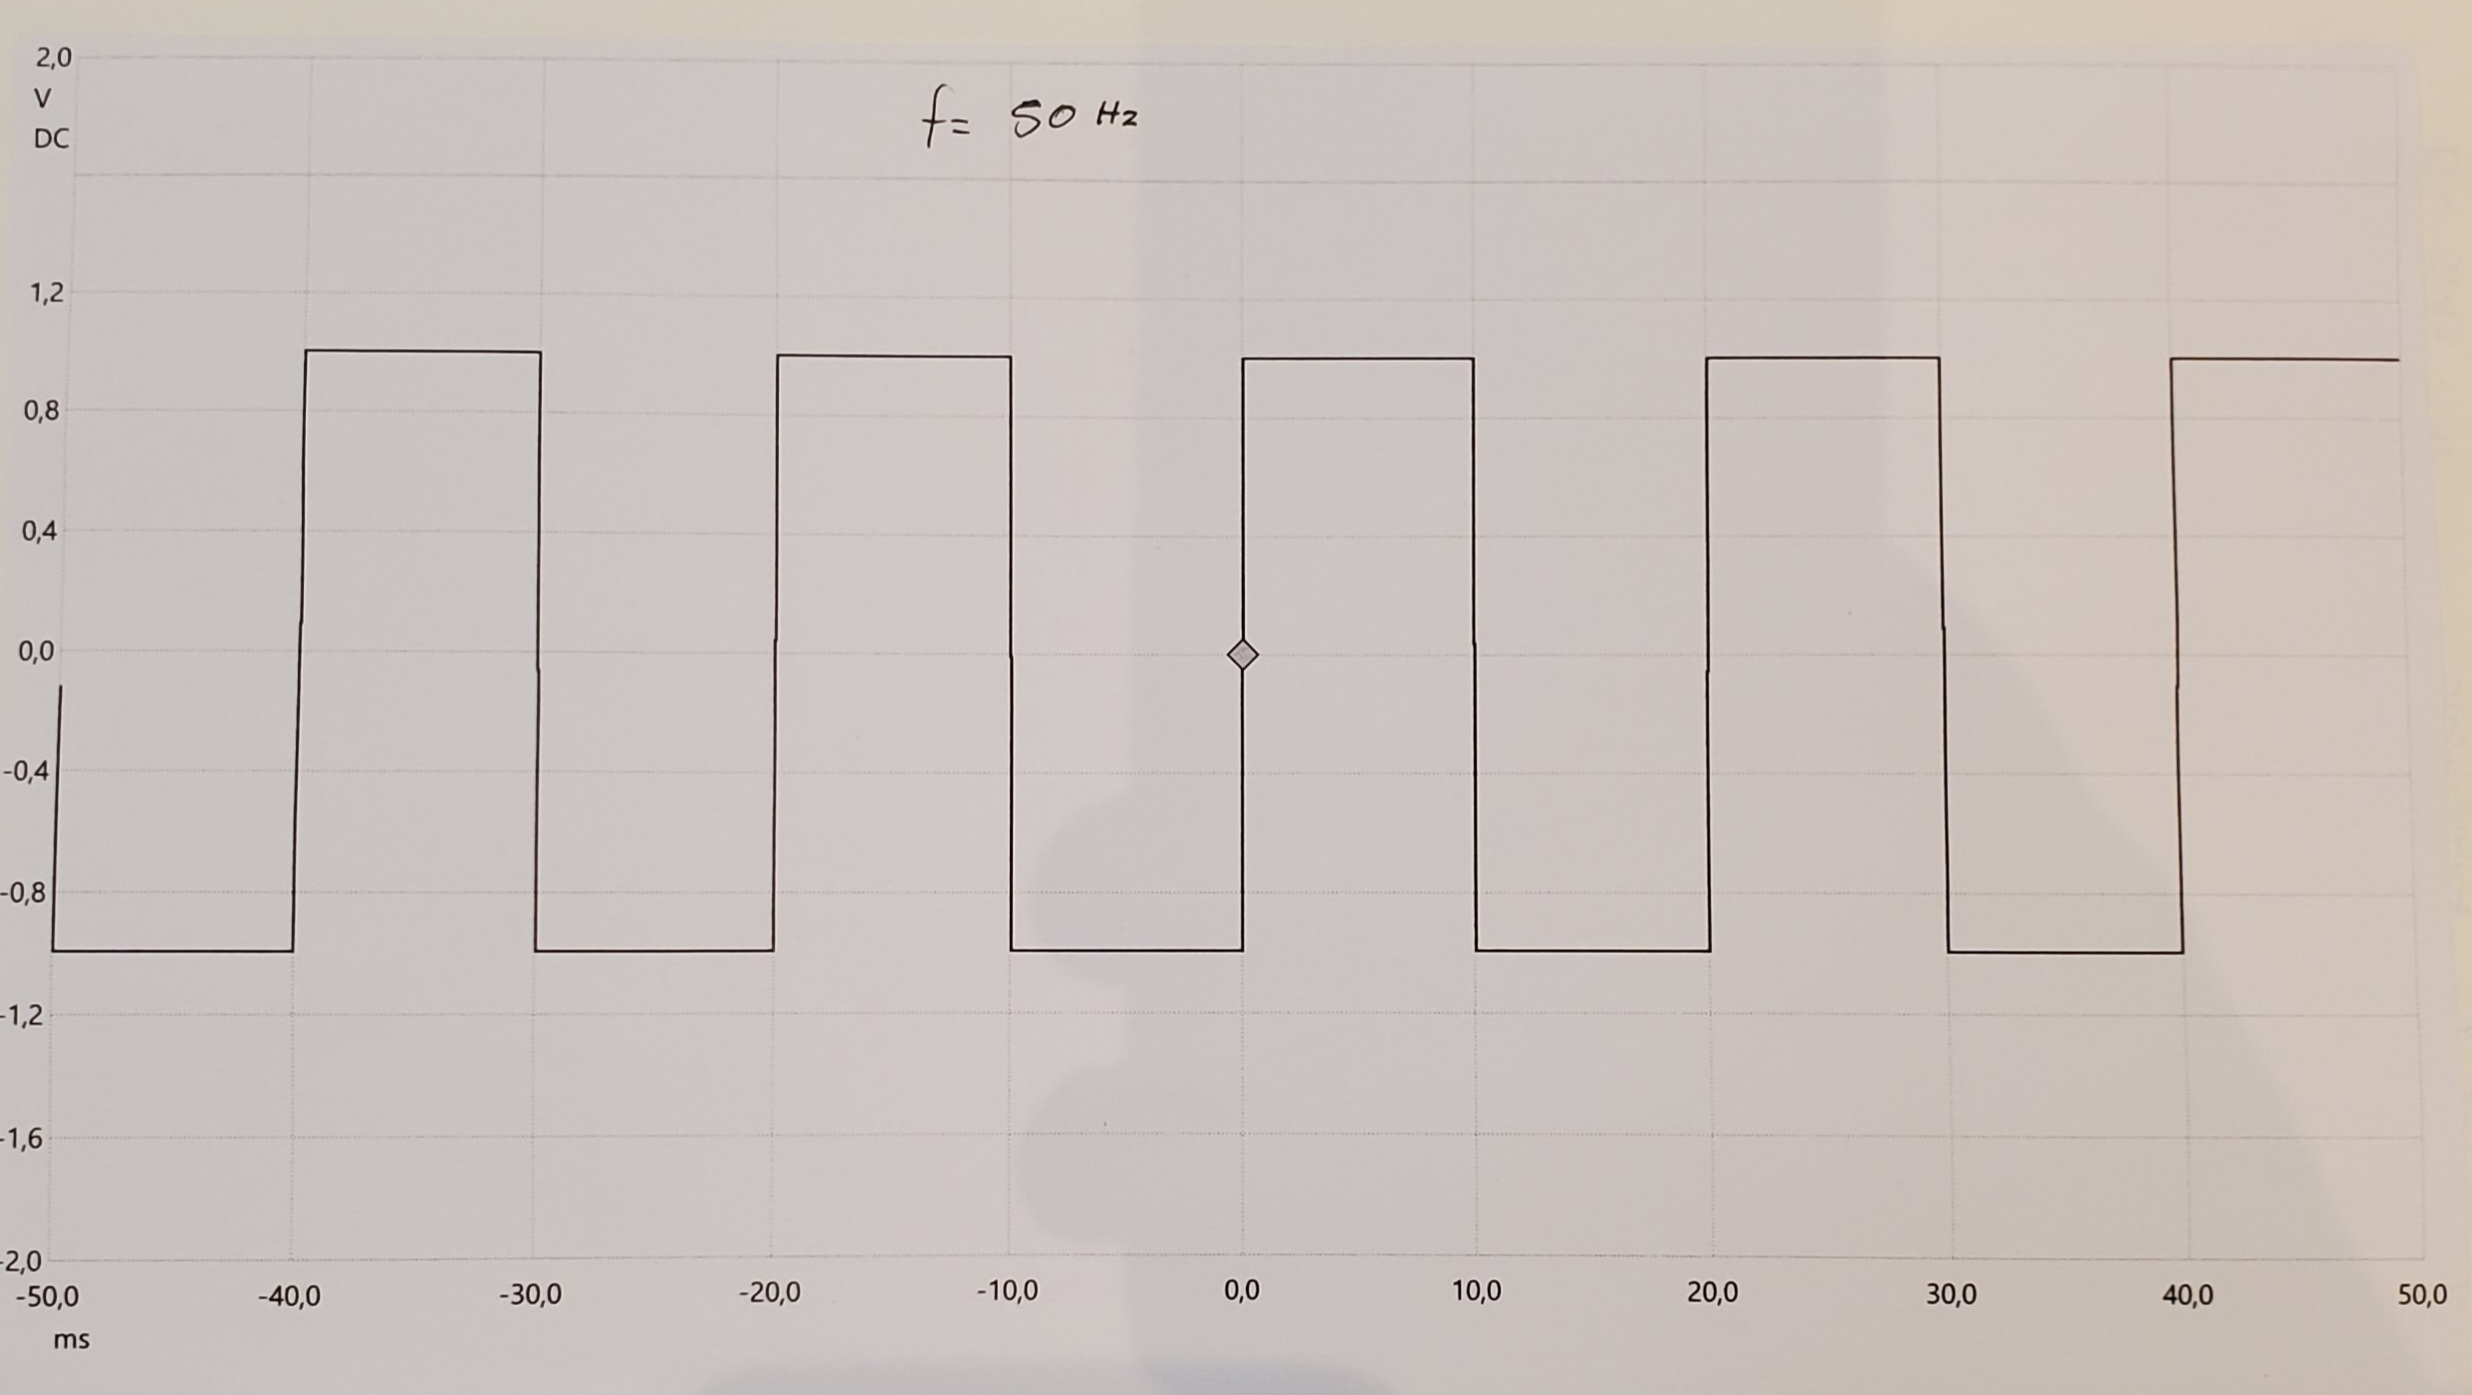
\includegraphics[width=1\textwidth]{Figs/firkantsignal.jpg}
    \caption{Firkantsignal som vist i PiscoScope 6 ved 1 volt og frekvens lik 50 Hz. Spenning(V) mot tid(ms). Oppgave 1. }
    \label{fig:sq_wave}
\end{figure}



\subsection{Del2}
I den andre delen ønsker vi undersøke flere deler. Først prøver vi å regne ut lengden på kobbertråden som igjen brukes til å finne en verdi av induktansen ved likning \ref{eq: induktansen}. Vi måler først resistansen i induktoren som er lik $5.6 + \pm 0.23 \Omega$. Måler lengden på coilen til 2.9cm og bruker likning \ref{eq: errorGange} der vi antar en avlesningsfeil på 0.1mm og nøyaktighet på 0.05mm. Som gir relativ feil på 0.1\%. \\ 

Deretter finner vi lambda, lengde på tråden, ved å dele motstanden på oppgitt verdi k. Igjen bruker likning \ref{eq: errorGange} for å finne sammensatt feil. Ender da opp med $\lambda = 15.8 \pm 0.6 m$. Til setter vi inn lambda i likning \ref{eq: induktansen} og finner at induktansen $0.86 \pm 0.07$ mH, hvor igjen på lik måte finner usikkerheten hvor A er usikkerhet til lambda og B er usikkerhet til lengden av coilen. Bruker minste gjeldende siffer fra måling av resistans (2 siffer).\\

Videre ønsker vi bruke en annen metode til å finne L. Ved måling av spenningen over begge komponenter og bare over resistoren kan vi bruke lineær regresjon til å finne en tilnærmet verdi. Verdiene avlest er vist i tabblen \ref{tab:dataLinReg}. Tar i bruk lineærregresjon ut i fra likning \ref{eq: V_a over V_r}, bare flytter 1 til andre siden. Linjen er vist i figur \ref{fig:linreg}. Grunnet veldig store avvik for spesielt siste punkt, men også nest siste, gjorde vi et valg etter råd fra veiledere å zoome inn på de fire første. Bruker innebygd scipy linreg funksjon og henter verdier for stigningstall og konstantledd. Får stigningstall like 52.9e-12 og et konstantledd lik -0.77. Finner L ved a trekke ut stigningstallet a som $\frac{L^2}{R^2}$, slik at $L = \sqrt{a}R$. Tilsvarende for å finne usikkerhet til L setter vi inn standard feil for a, som vi henter fra funksjonen i scipy linreg. Verdien for $L = 0.77 \pm 0.11 mH$. \\

Vi har nå to ulike verdier for L. For å finne den sammensatte usikkerheten bruker vi likning \ref{eq: errorPluss} som gir oss en usikkerhet lik 0.17 mH. Vi noterer oss at forskjellen mellom induktansene som er estimer er lik 0.09 mH, noe som er mindre enn usikkerheten.   \\

\begin{table}[htbp]
    \centering
    \caption{Data for måling av spenninger, frekvens og faseskift. $V_a$ er spenning over hele kretsen. $V_r$ også kalt for $V_b$ er spenning over resistor. Fasen er faseskiftet mellom $V_a$ og $V_r$ }
    \begin{tabular}{cccc}
    \hline
    \textbf{Frekvens $f$ [Hz]} & \textbf{$V_a$[mV]} & \textbf{Voltage $V_r$ [mV]} & \textbf{Fase [grader]} \\
    \hline
    $400$ & $107.6$ & $101$ & $1.78$ \\
    \hline
    $10\,000$ & $114.4$ & $100.7$ & $19.9$ \\
    \hline
    $50\, 000$ & $227.2$ & $97.84$ & $62.83$ \\
    \hline
    $100\, 000$ & $387.6$ & $89.31$ & $74.36$ \\
    \hline
    $200\, 000$ & $576.5$ & $62.8$ & $81.71$ \\
    \hline
    $300\, 000$ & $584.8$ & $35.5$ & $81.38$ \\
    \hline
    $400\, 000$ & $496.8$ & $14.18$ & $82.62$ \\
    \hline
    \end{tabular}
    
    \label{tab:dataLinReg}
\end{table}

\begin{figure}[htbp]
    \centering
    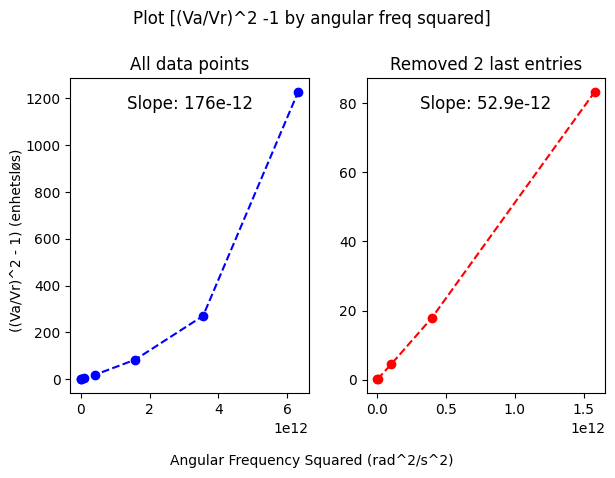
\includegraphics[width=1\textwidth]{Figs/linreg.png}
    \caption{Lineærregregresjon av dataene i tabell \ref{tab:dataLinReg} ved bruk av funksjonen stats.linregress i pakken scipy. Plotter dataene omformet til funksjonen: \ref{eq: V_a over V_r}. Bruker stigningstallet til å finne L.}
    \label{fig:linreg}
\end{figure}


Til slutt undersøker vi effekten. Vi velger åtte verdier for frekvens fra 5kHz til 80kHz og noterer likestrømgjennomsnittet til spenningene multiplisert vist i Pico programmet. Dataene er vist i tabell \ref{tab:effekt}. Undersøker om dataene stemmer overens som vi kan regne ut ved likning \ref{eq: P_snitt} , der vi tar i bruk cos til fasen. Plotter punkter der frekvenser overlapper som vist i figur \ref{fig:effekt}

\begin{table}[htbp]
    \centering
    \caption{Frekvens mot effekt gjennomsnitt. Går inn på verktøy/mattekanaler og velger $A*B$ i oscilloskop, velger deretter måling likestrømgjennomsnitt.}
    \begin{tabular}{ccc}
    \hline
    \textbf{Frekvens $f$ [Hz]} & \textbf{Effekt avg $P\_ snitt$ [W]} \\
    \hline
    $5 000$ & $10.77$ \\
    \hline
    $20 000$ & $10.69$ \\
    \hline
    $30 000$ & $10.61$ \\
    \hline
    $40 000$ & $10.48$ \\
    \hline
    $50 000$ & $10.32$ \\
    \hline
    $60 000$ & $10.13$ \\
    \hline
    $70 000$ & $9.90$ \\
    \hline
    $80 000$ & $9.646$ \\
    \hline
    \end{tabular}
    \label{tab:effekt}
\end{table}


\begin{figure}[htbp]
    \centering
    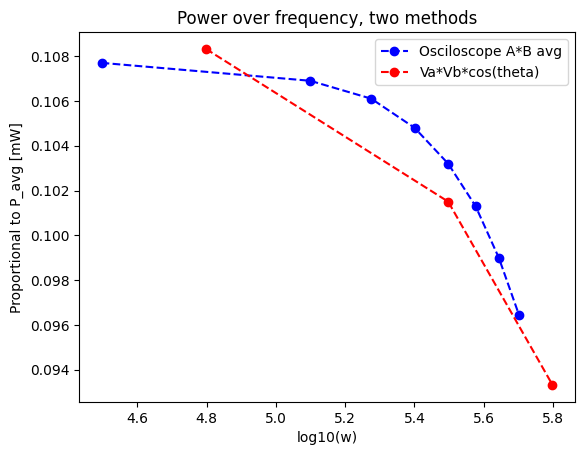
\includegraphics[width=1\textwidth]{Figs/effektavsettning.png}
    \caption{Viser gjennomsnitt til effekten mot vinkelfrekvensen(logaritmisk skala). Røde linjen viser 3 spenningener multiplisert med cos til fasen hentet fra tabellen \ref{tab:dataLinReg}. Blå linjen viser verdien likestrømgjennomsnitt for Va*Va delt på resistansen i motstanden (100 ohm).}
    \label{fig:effekt}
\end{figure}



\section{Diskusjon}
\subsection{Del 1}
I første del hvor vi måler RMS verdien ser vi at for Picoskopet stemmer de målte verdiene perfekt opp mot de de teoretiske verdiene. For sinus får vi 0.707V (vist i likning \ref{eq: RMSsin}) og for firkant blir det ca like 0.997 (vist i likning \ref{eq: RMSsq}). Vi ser at sinus signalets RMS holder seg konstant, men for firkant minker det minimalt ved høyere frekvens. Grunnen kan ligge i at boksen ikke klarer å lage et signal med perfekt verdi av spenning ved høyere frekvenser. En annen grunn er at i firkant bølge vil vi ideelt gå fra V0 til 0 momentant, men er ikke mulig i praksis. Så når vi øker frekvensen vil det øke bidraget fra overgangene. Det er også mulig at instrumentet er mer kalibrert for sinus bølger, siden det er det som mest tas i bruk.

For multimeteret ser vi at i begge tilfeller vil den målte verdien synke ved høyere frekvenser. Spesielt etter 1khZ. Dette er grunnet i at multimeteret tar i bruk en "bridge rectifier" som konverterer AC til DC. Det er en kapasitans på innsiden som er lagd med tanke på dagligdags bruk for frekvenser rundt 45-500Hz. Ved de høyeste frekvensene klarer ikke kapasitansen å lade eller utlade i tide som fører til for lav målt verdi av spenningen.

For måling av en DC-komponent lagt til i kretsen kan vi ta i bruk multimeteret eller oscilloskopet. Ved å sette multimeteret på instillingen DC vil vi bare måle DC-delen av kretsen. For oscilloskopet kan vi legge til måling av likestrømgjennomsnittet i Pico programmet.


\subsection{Del 2}
Vi finner induktansen på to ulike måter. Forskjellen er mindre enn den totale feilen. Dette viser at antagelsen vi har gjort når vi finner likning \ref{eq: induktansen} stemmer relativt godt overens med de målte dataene.

Konstantleddet om induktoren hadde vært perfekt ville vært 0, vi fikk et konstantledd på -0.77 som indikerer at det ikke er en helt ren induktor. Ellers passer linjen godt til punktene og vi får liten relativ feil. Viktig å nevne at vi valgte å fjerne de to siste punktene for lineærregresjonen ettersom de blåste opp modellen. Inkludert alle punkter  L hadde doblet og feilen vært på 0.54mH, som er omtrent lik verdien L i seg selv. Induktoren vil oppføre seg som en resistor ved lave frekvenser, på ca 5\% av kresen. Ikke mulig å få en perfekt induktor siden kobbertråden har innebygd resistans. Eneste måten å få tilnærmet perfekt induktor er hvis vi bruker en superleder, som har null resistans.

Videre undersøkelsen av effekt gjennomsnitt ser vi at når vi øker frekvensen så øker faseforskyvningen. Siden effekten er proporsjonal med spenningene multiplisert ser vi at produktet minker når fasen går mot 90 grader. $P = \frac{V^2}{R} = V_a * V_r$, hvor $V_r = I_r/R$ for en resistor. Effekten vil i et øyeblikk kunne være negativ, siden f.eks spenningen kan være positiv og spenning være negativ. Dette betyr ikke at energi blir tilintetgjort eller oppstår fra ingenting. Den er lagret i induktorens magnetfelt. Den tar opp energi når strømmen øker og slipepr fra seg når strømmen minker. Ved negativ effekt viser det til tiden hvor induktoren slipper fra seg energi. Viktig å nevne at gjennomsnitt over lengre tid vil alltid være større enn null grunnet resistansen i induktoren og resistoren. Dette er viktig for å forstå effekten i kretser hvor vi har induktive komponenter som i elektriske motorer og transformatorer. 

Til slutt fant vi ut at likestrømgjennomsnitt til de to multipliserte spenningene og tallene ved bruk av cos til vinkel stemmer omtrent overens. Vi ser at ved økning av frekvens vil effekt gjennomsnittet minke eksponentielt i forhold til logaritmisk skala for vinkelfrekvensen.

\section{Konklusjon}

Ved hjelp av en enkel krets med en induktans og motstand fant vi at multimeteret hadde problemer med frekvenser høyere enn 500-1000Hz. Oscilloskopet var veldig presist i forhold til den teoretiske verdien for sinus, men var litt mindre for firkantbølge. Kan være på grunn av firkantbølgens bratte former og instrumentet kan være kalibert spesielt for sinusbølger. Vi brukte diverse formler og lineærtilpasning for å finne en induktans lik 0.86 og 0.77. Med en total usikkerhet på 0.17, ligger verdiene bare 0.09 mH fra hverandre. Dette kan gi mening med tanke på at første verdi antar ideell induktor med null resistans og verdiene er fortsatt innenfor den totale usikkerheten. Til slutt fant vi at gjennomsnittet av effekten ,gjennom to ulike måter å bergenge effekt på, går mot 0 med økende frekvens. Detter er på grunn av at faseforskjellen øker mellom spenningen og strømmen. Maksimum 90 grader, men vil i praksis aldri nå helt dit siden induktoren har innebygd resistans på 5.6 ohm som målt tidligere.


\bibliography{referanser}
% legg til refereanse til teori om induktans, reaktans, impedans etc. SNL

\newpage
\begin{appendices}
\section{Skjema for oppgave 1}
\begin{figure}[htbp]
    \centering
    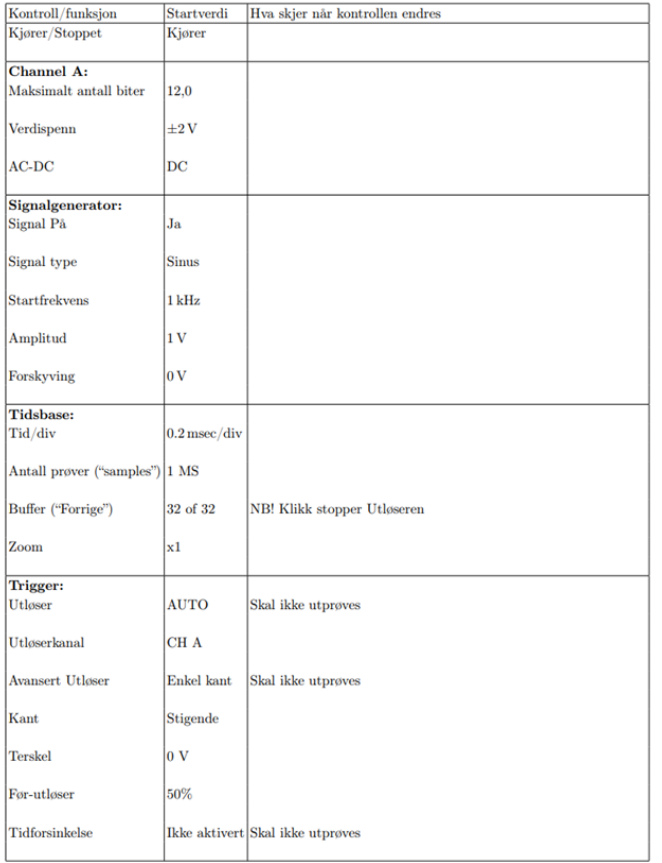
\includegraphics[width=0.9\textwidth]{Figs/FYS2150_lab1.png}
    \label{fig:appendiksA}
\end{figure}
\end{appendices}


\begin{appendices}
\section{Jupyter Notebook}
I forbindelse med de beregninger og analyser som presenteres i denne rapporten, har all kildekode og interaktive beregninger blitt implementert i en Jupyter Notebook. 
\end{appendices}
\end{document}
